%%%%%%%%%%%%%%%%%%%%%%%%%%%%%%%%%%%%%%%%%%%%%%%%%%%%%%%%%%%%%%%%%%%%%%%%%%%%%%%%%%%%%%%%%%%%%%%%
%
% CSCI 1430 Final Project Report — Sailboat Pose Estimation
%
%%%%%%%%%%%%%%%%%%%%%%%%%%%%%%%%%%%%%%%%%%%%%%%%%%%%%%%%%%%%%%%%%%%%%%%%%%%%%%%%%%%%%%%%%%%%%%%%

\documentclass[10pt,twocolumn,letterpaper]{article}

\usepackage{cvpr}
\usepackage{times}
\usepackage{epsfig}
\usepackage{graphicx}
\usepackage{amsmath}
\usepackage{amssymb}
\usepackage{booktabs}
\usepackage{microtype}
\usepackage[numbered,framed]{matlab-prettifier}

\frenchspacing

\usepackage[pagebackref=true,breaklinks=true,letterpaper=true,colorlinks,bookmarks=false]{hyperref}

\cvprfinalcopy
\def\cvprPaperID{****}
\def\httilde{\mbox{\tt\raisebox{-.5ex}{\symbol{126}}}}
\ifcvprfinal\pagestyle{empty}\fi

\begin{document}

%%%%%%%%% TITLE
\title{CSCI 1430 Final Project Report:\\Sailboat Pose Estimation from Drone Footage}

\author{
    \emph{Team name}: Quinn Brighton, Nishani Clarke, Alexandra McIntyre.\\
    \emph{TA name:} Kelvin Jiang.
    Brown University\\
}

\maketitle

%%%%%%%%% ABSTRACT
\begin{abstract}
We present an end-to-end pipeline that turns a monocular sailing-race broadcast into metric per-frame camera pose and per-boat $(x, y, \mathrm{yaw})$ in world coordinates, with no calibration and no GPS.  A frozen DINOv3 ViT-S/16 backbone supplies dense image features to three small CNN heads that predict four semantic keypoints per boat --- mast tip, mast base, bow, and stern --- in a staged conditioning cascade (tip $\rightarrow$ base $\rightarrow$ bow/stern).  These detections feed a single-frame least-squares solver that jointly fits camera intrinsics/extrinsics and per-boat $(x, y, \mathrm{yaw}, \mathrm{heel})$ to a known sailboat hull/mast template; an iterative outlier-rejection step prunes occluded keypoints before the final fit.  On a held-out 43-second section of the source race the pipeline solves \textbf{172 of 172 frames (100\%)} with a \textbf{median reprojection RMS of 3.88\,px} and a \textbf{maximum of 6.18\,px} on 1080p imagery --- well below our 15\,px target.  The pipeline is one shell script: it downloads a section of YouTube, extracts frames, runs inference, writes per-frame solves, and renders a metric top-down view of the race.
\end{abstract}

%%%%%%%%% BODY TEXT
\section{Introduction}

Major professional sports leagues have adopted spatial tracking analytics to study positioning and tactics, but collegiate sailing has no comparable system.  Coaches collect hours of drone or broadcast footage from regattas and review it manually; converting that footage into a quantitative top-down view of fleet movement is precisely the kind of perception problem that off-the-shelf computer-vision tools should be able to solve.

The challenges are non-trivial.  Boats appear at widely varying scales; water reflections, wakes, and overlapping sails confuse generic detectors; the camera itself is constantly zooming and panning with no calibration available; and there is no GPS ground truth to anchor the result.  Estimating both boat pose and camera pose simultaneously from a single uncalibrated frame is an underconstrained problem in general.

Our approach is to combine a strong self-supervised visual backbone with a small amount of task-specific supervision and a tightly-engineered geometric solver.  We use a frozen DINOv3~\cite{Oquab2023} Vision Transformer to produce dense per-pixel features, train three lightweight neural heads to extract four semantic keypoints per visible boat (mast top, mast base, bow, stern), and then drop the detections into a per-frame least-squares optimisation that fits a known rigid sailboat template under a pinhole camera.  The metric scale of the template is what gives us metric world coordinates without any calibration.

We show that this combination produces stable, sub-7-px per-frame reprojection error on a held-out clip --- accurate enough that the recovered camera pose plus boat positions reproject cleanly back onto the original frame, and accurate enough to render an interpretable top-down view of the race directly from the per-frame solves.

\section{Related Work}

\paragraph{Self-supervised visual backbones.}
We build on DINOv3~\cite{Oquab2023}, whose dense patch embeddings separate sails, hulls, and water far better than ImageNet-supervised backbones, even on aerial crops never seen during pretraining.  Frozen self-supervised features paired with small task heads have repeatedly been shown competitive with full fine-tuning for downstream perception.

\paragraph{Keypoint-based pose estimation.}
Our solver follows the perspective-$n$-point tradition: given image keypoints with known 3D correspondences, recover camera and object pose by minimising reprojection error~\cite{Hartley2003}.  Where standard PnP assumes calibrated intrinsics, we treat focal length as a free per-frame variable and rely on the multi-boat geometric constraint to make the problem identifiable.  For outlier handling, we use the simplest robust option: after each least-squares pass, drop the worst-fitting keypoint above a fixed pixel threshold and re-solve.

\section{Method}

Our goal is to recover a metrically-scaled top-down representation of a sailing race from monocular footage.  The system has two major stages: (1) a learned keypoint detection pipeline built on frozen DINOv3 features, and (2) a per-frame geometric solver that reconstructs the scene from those keypoints.

\subsection{DINOv3 Feature Extraction}

We use the \texttt{facebook/dinov3-vits16-pretrain-lvd1689m} ViT-S/16 model as a frozen feature extractor.  Each input frame is resized so the longest dimension is at most 1808\,px and both spatial dimensions are divisible by 16, then normalised with ImageNet statistics.  We modify the patch-embedding stride from 16 to 8, producing overlapping patches and a denser spatial feature grid --- this materially improves localisation of small structures like masts.  After inference, the transformer tokens are reshaped into a dense feature tensor
\begin{equation}
F \in \mathbb{R}^{H \times W \times 384},
\end{equation}
where each spatial cell carries a normalised 384-dimensional embedding.  The same $F$ feeds all three downstream heads.  Figure~\ref{fig:dinov3} shows a PCA projection of $F$: sails, hulls, and water are clearly separated even though the backbone has never been fine-tuned on sailing.

\begin{figure}[t]
    \centering
    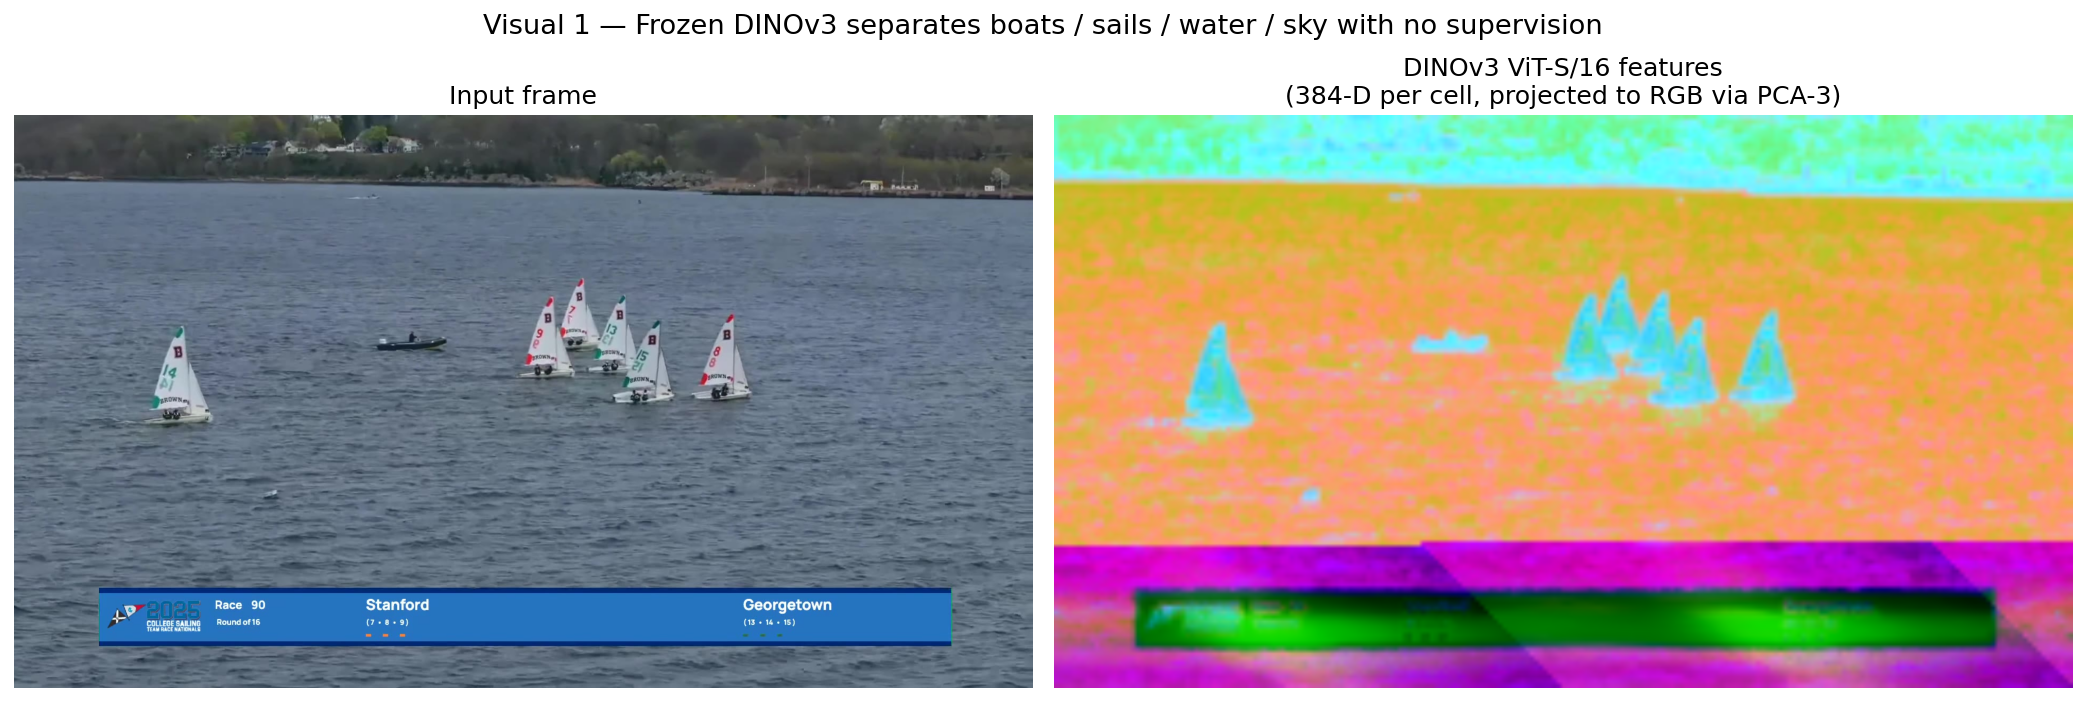
\includegraphics[width=\linewidth]{visual/01_dinov3_features.png}
    \caption{Top-3 PCA components of the frozen DINOv3 ViT-S/16 stride-8 feature map on a held-out frame.}
    \label{fig:dinov3}
\end{figure}

\subsection{Stage 1: Mast Tip Detection}

The first head, \texttt{TileHead}, is a four-layer fully-convolutional network that runs on local windows of $F$ and predicts a per-cell mast-tip probability heatmap.  At inference time it slides densely across the feature grid; the local heatmaps are merged into a global confidence map and clustered with DBSCAN to produce a final set of tip detections, which are then mapped back into source-image pixel coordinates.

\begin{figure}[t]
    \centering
    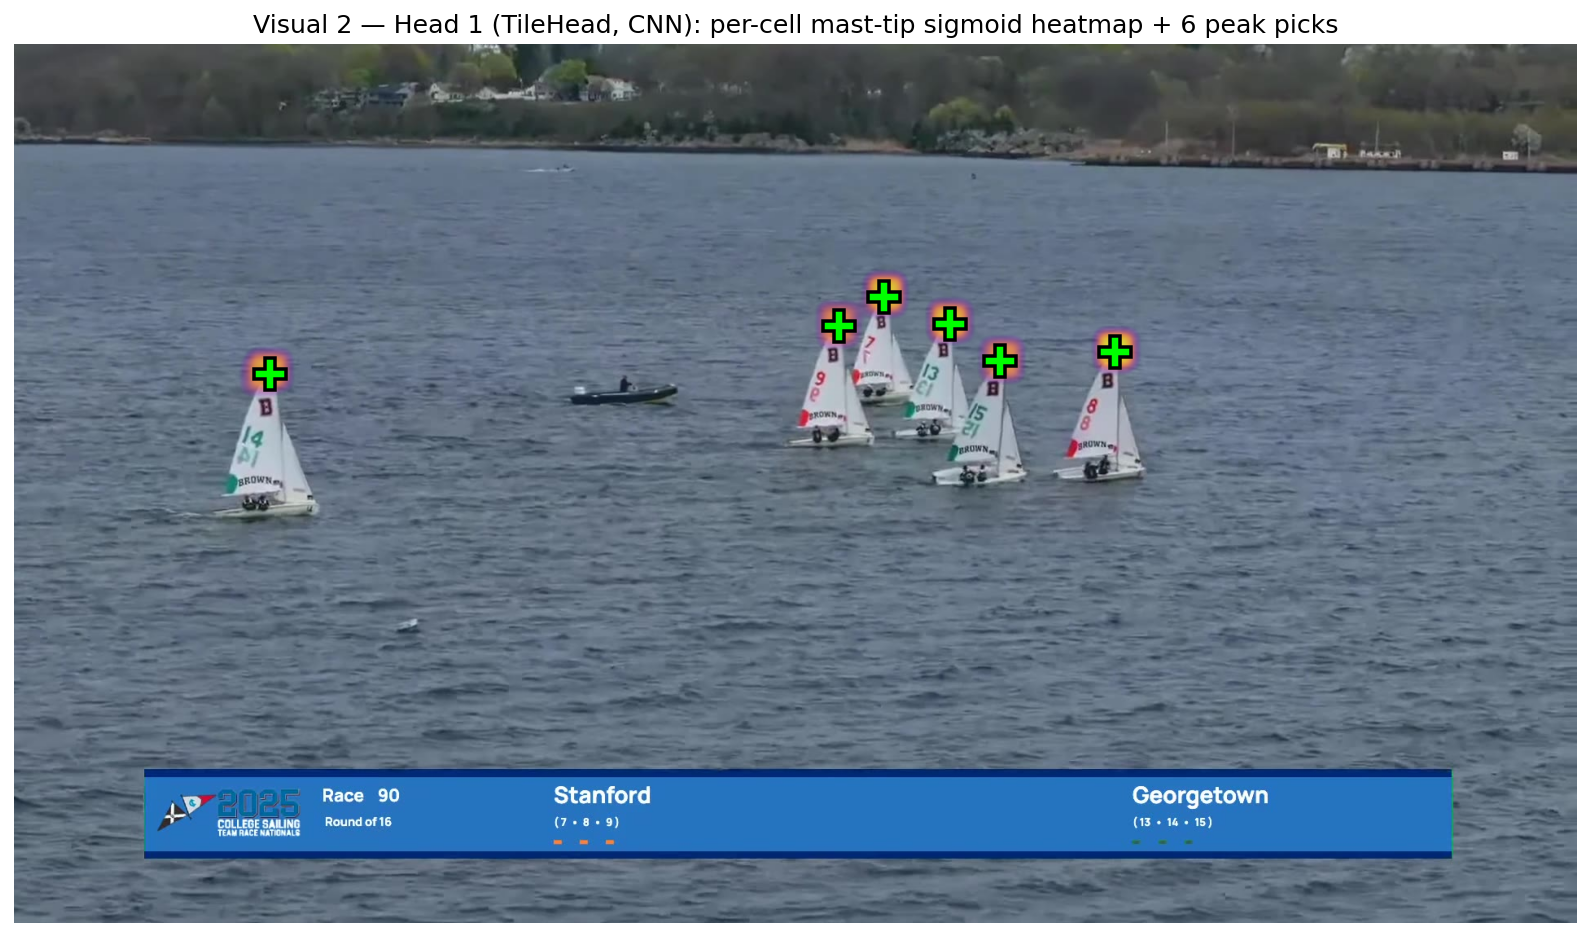
\includegraphics[width=\linewidth]{visual/02_tip_heatmap.png}
    \caption{Mast tip detection heatmap.  Peaks correspond one-to-one with visible mast tops, regardless of zoom or boat orientation.}
    \label{fig:tipheat}
\end{figure}

\subsection{Stage 2: Tip-Conditioned Mast Base Prediction}

Given a detected mast tip, the second head, \texttt{TipAttnBaseHead}, predicts the corresponding mast base.  This task spans larger pixel distances than tip detection and benefits from explicit spatial reasoning.  For each tip we extract a $21 \times 34$-cell feature window centred on the tip, with the tip pinned at a fixed window position $(\text{row}=2, \text{col}=10)$.  The window features are projected into a 128-dim embedding, augmented with a 2D sinusoidal positional encoding, and processed through two transformer encoder layers (4 heads, GELU, pre-norm).  After self-attention, the tip-cell feature is concatenated with every spatial token, and a small MLP outputs a per-cell base-presence logit.  The output heatmap is converted to a sub-pixel base prediction via a weighted centroid around the maximum response.

\begin{figure}[t]
    \centering
    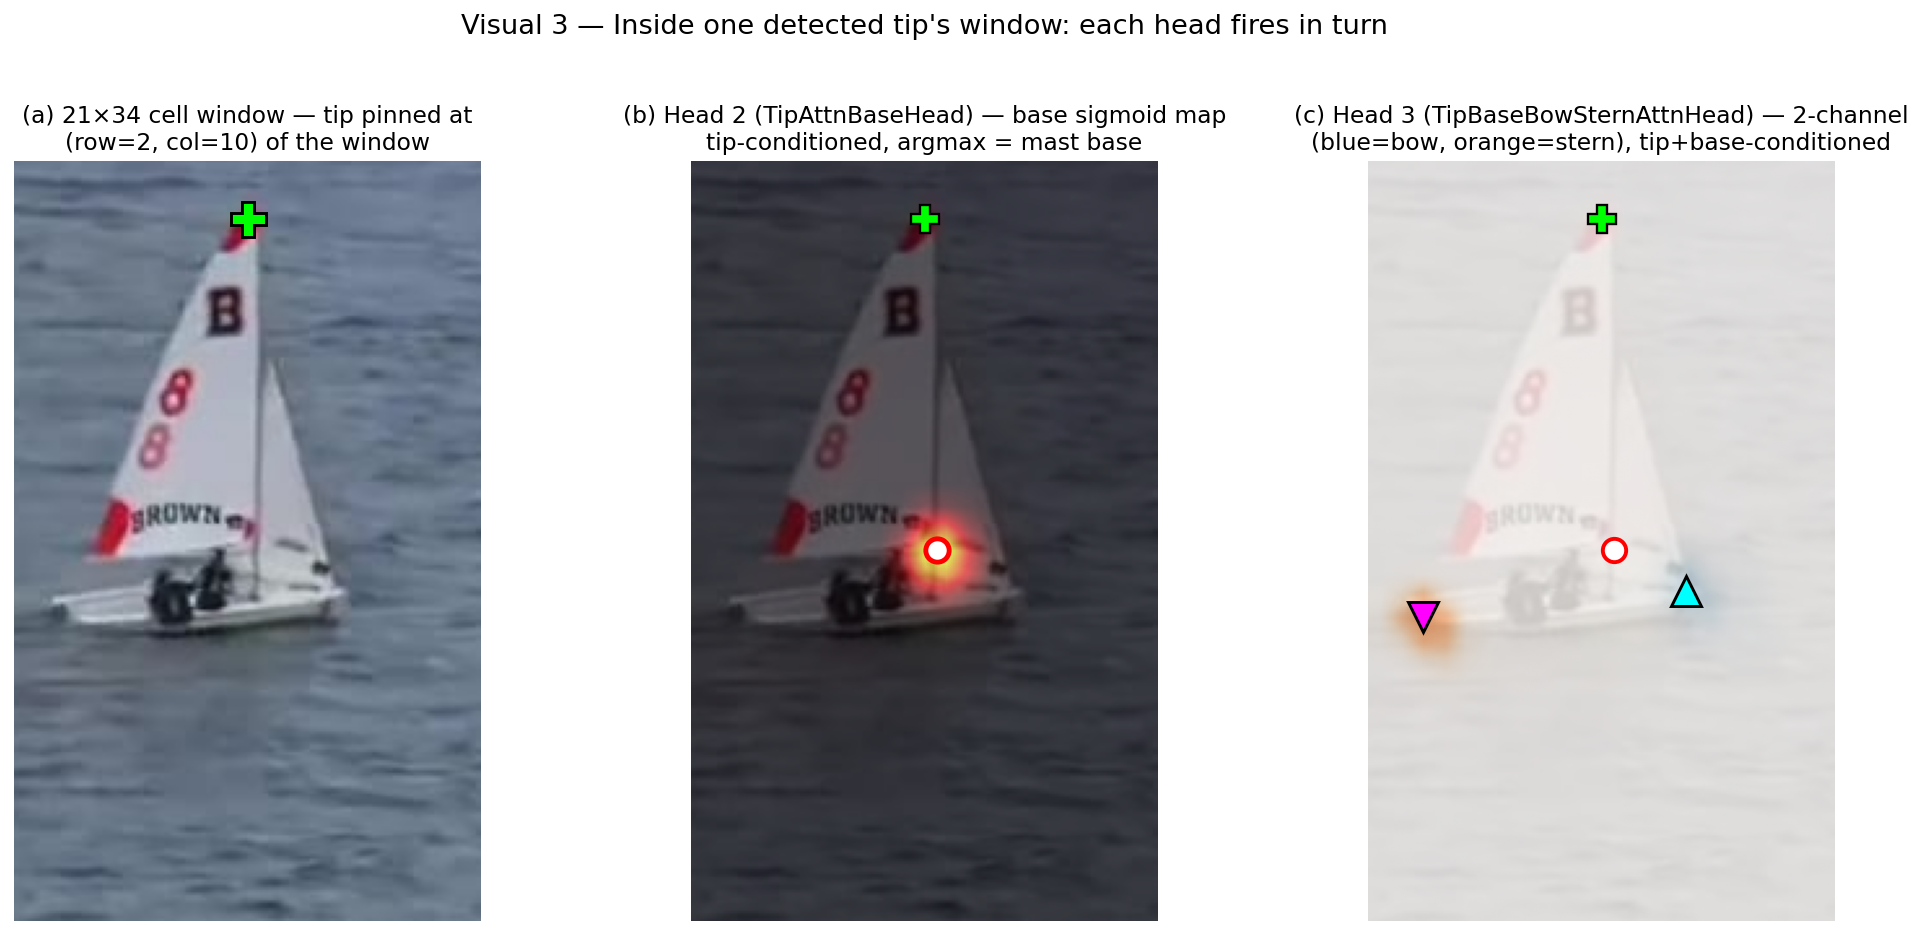
\includegraphics[width=\linewidth]{visual/03_window_panels.png}
    \caption{Local feature windows used by stages 2 and 3: a $21 \times 34$-cell DINOv3 window centred on each detected mast tip.}
    \label{fig:windows}
\end{figure}

\subsection{Stage 3: Bow and Stern Prediction}

The third head, \texttt{TipBaseBowSternAttnHead}, shares the stage-2 backbone but conditions on the mean of the post-attention features at both the tip cell and the (variable) base cell, and produces two output channels (bow + stern) in parallel.  Mast direction is informative for hull orientation and heel, so passing both keypoints in as conditioning signals materially stabilises bow/stern prediction.  For each detected boat the learned pipeline emits four image-space keypoints
\begin{equation}
K_i = \{ \mathbf{u}_{\text{bow}}, \mathbf{u}_{\text{stern}}, \mathbf{u}_{\text{base}}, \mathbf{u}_{\text{tip}} \}.
\end{equation}

\subsection{Single-Frame Geometric Solver}

The four keypoints per boat feed a per-frame least-squares solver that jointly estimates camera pose, intrinsics, and per-boat pose by minimising reprojection error against a rigid metric template.  The template uses dimensions of collegiate FJ/420 sailboats and places the four landmarks in a local boat frame as
\begin{align}
\text{bow}      &= (-L_h/3,\ 0,\ 0), &
\text{stern}    &= (+2 L_h/3,\ 0,\ 0), \\
\text{mastbase} &= (0,\ 0,\ 0.7), &
\text{masttop}  &= (0,\ 0,\ 0.7 + H_m),
\end{align}
with $L_h = 4.2$\,m hull length and $H_m = 5.2$\,m mast height.  Because the metric scale is baked into the template, the recovered scene is metric.  The world frame has the water surface at $z = 0$.

The unknowns are camera $(\text{pitch}, \text{yaw}, h, c_x, c_y, f)$ and per-boat $(x_i, y_i, \theta_i, \phi_i)$ where $\theta_i$ is the in-plane yaw and $\phi_i$ is the heel angle.  Each landmark is projected via a pinhole model:
\begin{equation}
\hat{\mathbf{u}}_{i,j} = \Pi(\mathbf{X}_{i,j}; \theta_{\text{cam}}, \theta_i^{\text{boat}}),
\end{equation}
and we minimise sum-of-squared reprojection error,
\begin{equation}
E_{\text{reproj}} = \sum_{i,j} \big\| \hat{\mathbf{u}}_{i,j} - \mathbf{u}_{i,j} \big\|_2^2,
\end{equation}
with a soft heel prior that weakly penalises large heel values when image evidence is weak.  Each frame is solved independently --- there is no temporal coupling across frames.  The multi-boat reprojection constraint is what makes the per-frame problem identifiable despite the unknown focal length.

\begin{figure}[t]
    \centering
    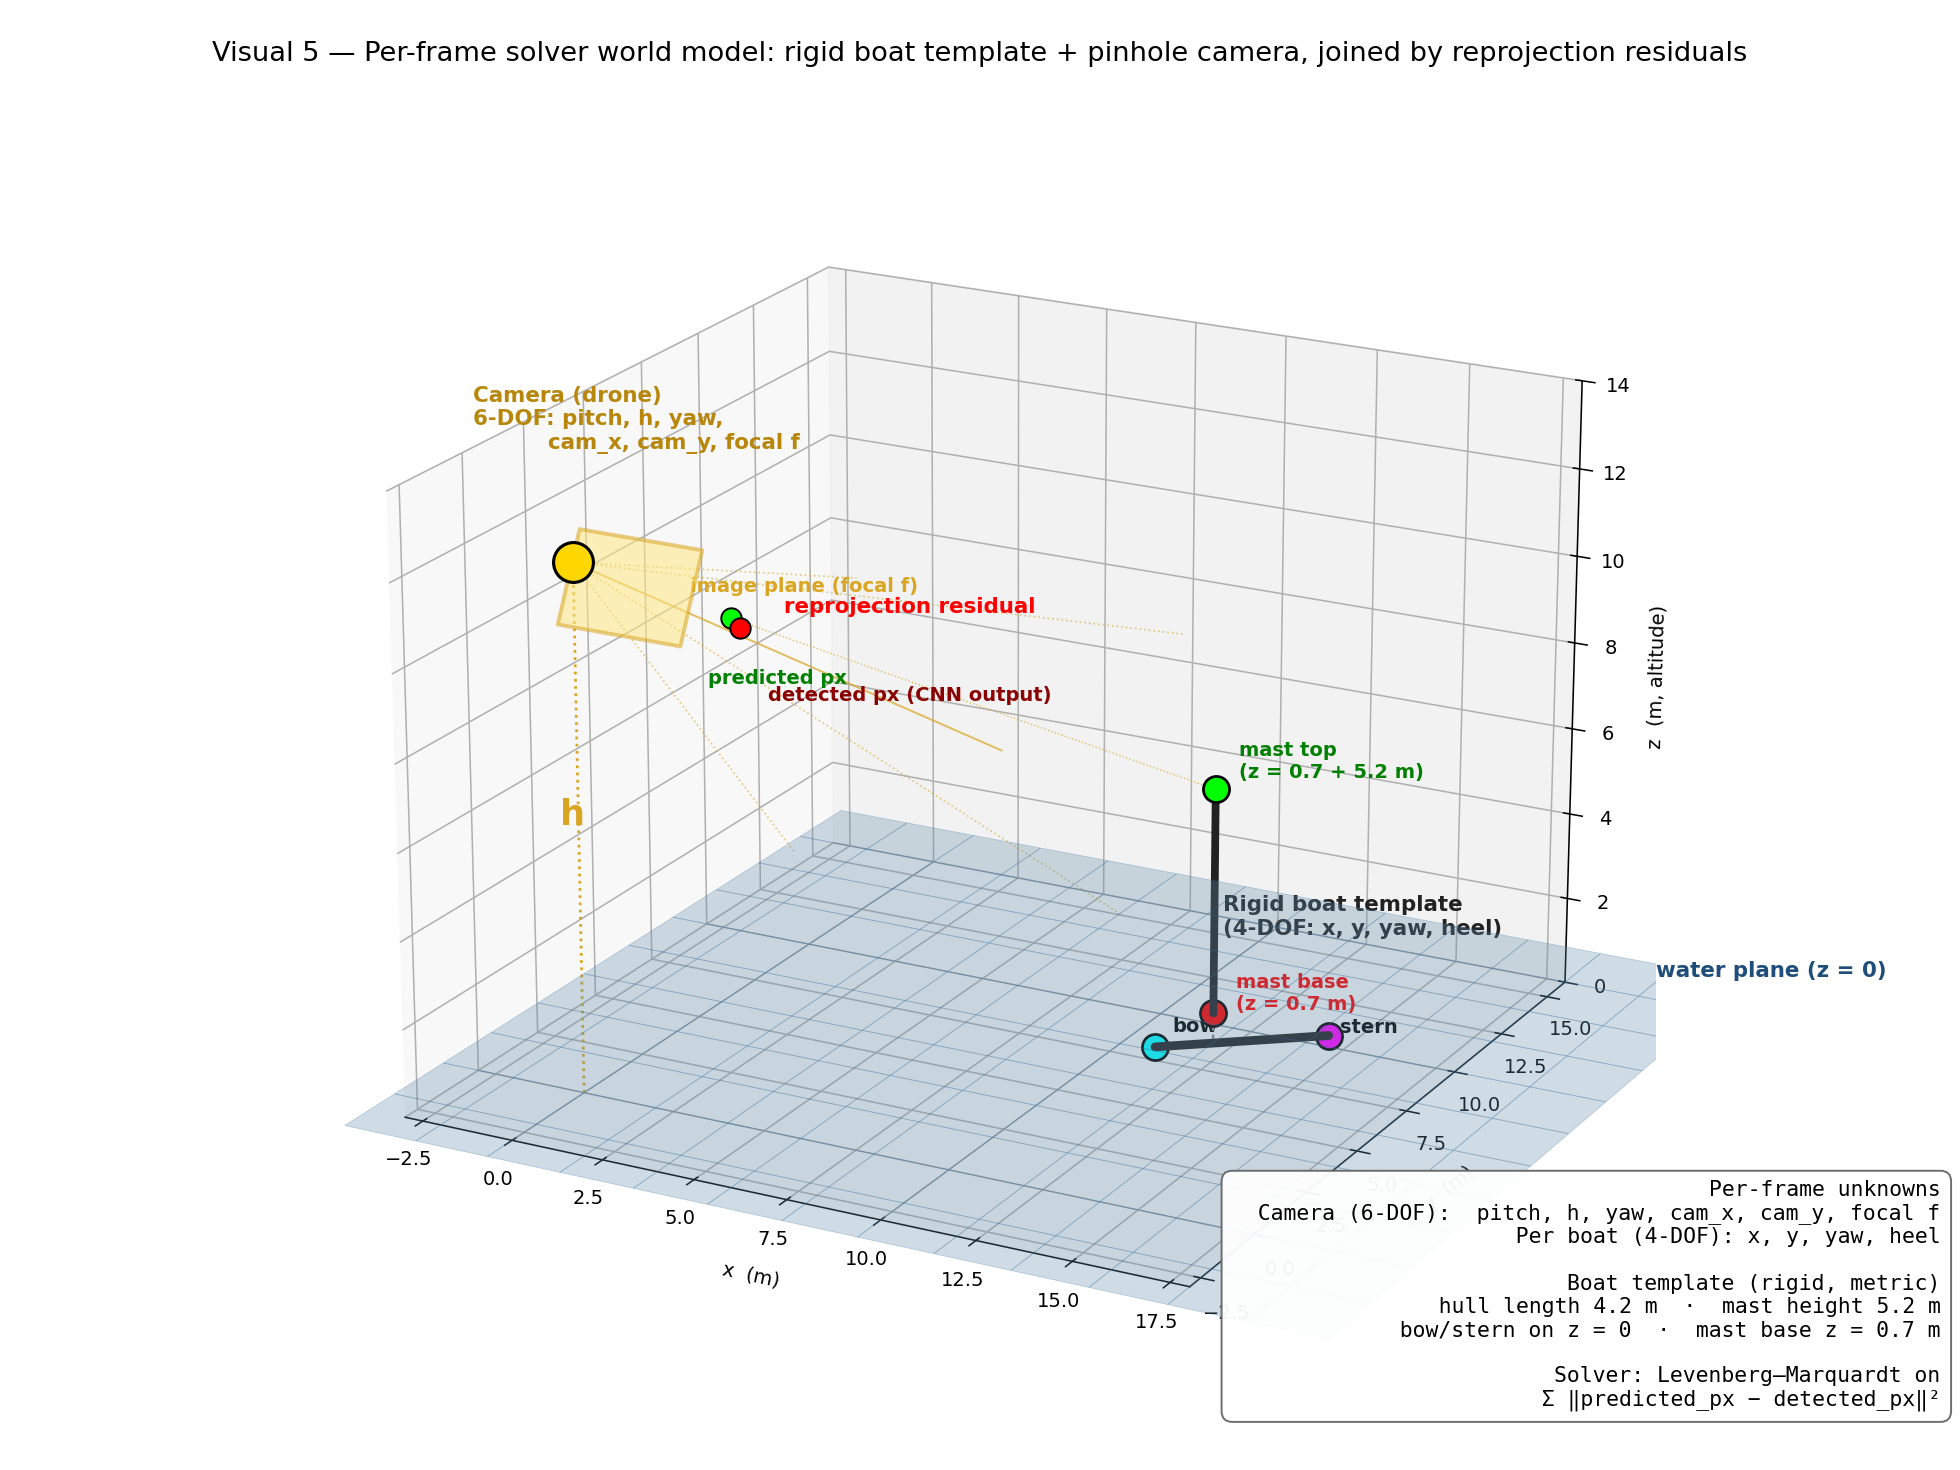
\includegraphics[width=\linewidth]{visual/05_solver_geometry.png}
    \caption{World-coordinate boat template ($L_h = 4.2$\,m hull, $H_m = 5.2$\,m mast).  The water surface is the plane $z = 0$.}
    \label{fig:solver-geom}
\end{figure}

\subsection{Iterative Outlier Rejection}

Predicted keypoints occasionally have large localisation errors due to occlusion, overlapping sails, or poor visibility.  After each least-squares pass we compute per-keypoint reprojection error; the worst keypoint above a 15-px threshold is dropped from the active set and the solver is re-run.  This continues until all surviving keypoints fall below the threshold or every boat reaches a minimum number of active landmarks.  A final pass with the heel prior re-enabled regularises any remaining ambiguity.

\section{Results}

We evaluated on a 43-second held-out section of the source race (YouTube 0:22 to 1:05) that the detector heads had not been trained on.  The default \texttt{run\_full\_pipeline.sh} downloads this section, extracts 172 frames at 4 fps, and runs the full inference and solver stack.

\subsection{Reprojection Accuracy}

\begin{table}[t]
\begin{center}
\begin{tabular}{l c}
\toprule
Metric & Value \\
\midrule
Frames solved          & 172 / 172 (100\%) \\
Median per-frame RMS   & \textbf{3.88\,px} \\
p25 / p75              & 3.48 / 4.46\,px \\
p90                    & 4.98\,px \\
Maximum                & \textbf{6.18\,px} \\
Frames over 15\,px     & 0 \\
\bottomrule
\end{tabular}
\end{center}
\caption{End-to-end results on the held-out 43-second clip (172 frames at 4 fps, 1080p).  Per-frame RMS reprojection error across all active keypoints.  Every solved frame fell below the 15-px target.}
\label{tab:results}
\end{table}

Table~\ref{tab:results} summarises the headline numbers.  Every frame in the test clip was solved, and every solve had per-frame RMS below 7\,px.  Of the 172 solved frames, 167 are below 5\,px and the remaining 5 fall between 5 and 7\,px.  An RTX 3060 processes the full 172-frame clip end-to-end in roughly half an hour, dominated by DINOv3 feature inference; the per-frame solver itself is fast.

\begin{figure}[t]
    \centering
    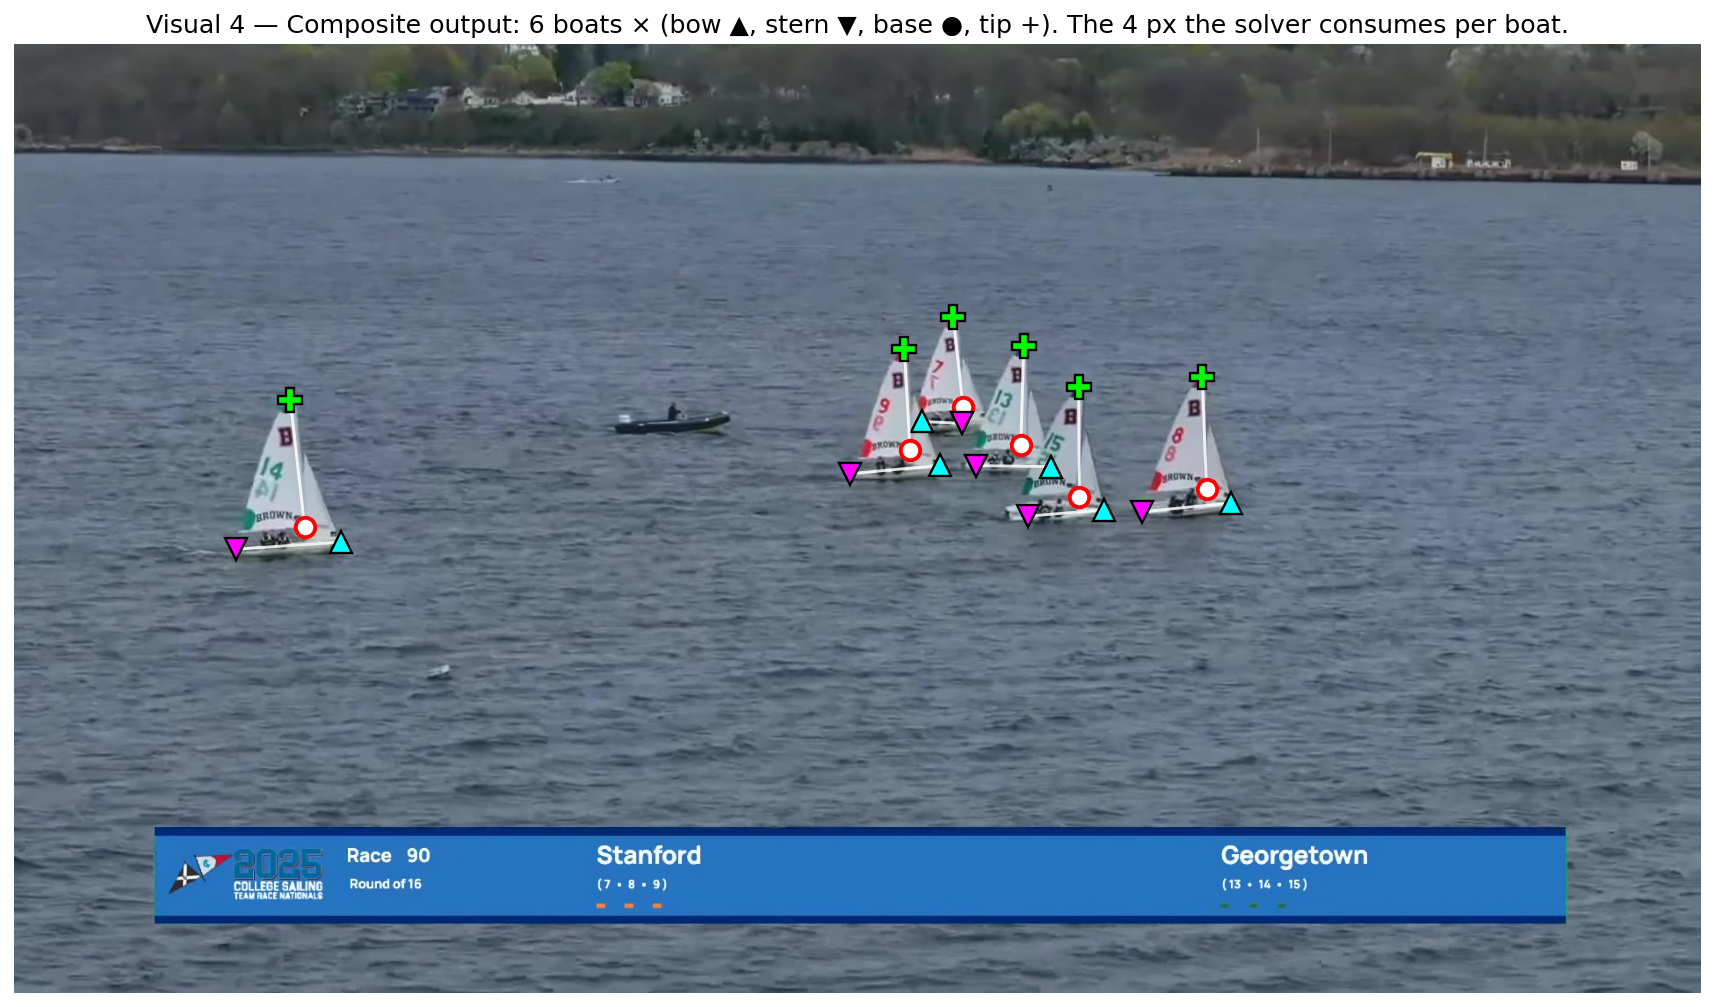
\includegraphics[width=\linewidth]{visual/04_composite_keypoints.png}
    \caption{Per-frame keypoint detections from the cascaded \texttt{TileHead} $\rightarrow$ \texttt{TipAttnBaseHead} $\rightarrow$ \texttt{TipBaseBowSternAttnHead} stack: bow (red), stern (blue), mast base (green), mast tip (yellow) overlaid on a held-out frame.}
    \label{fig:result1}
\end{figure}

\begin{figure}[t]
    \centering
    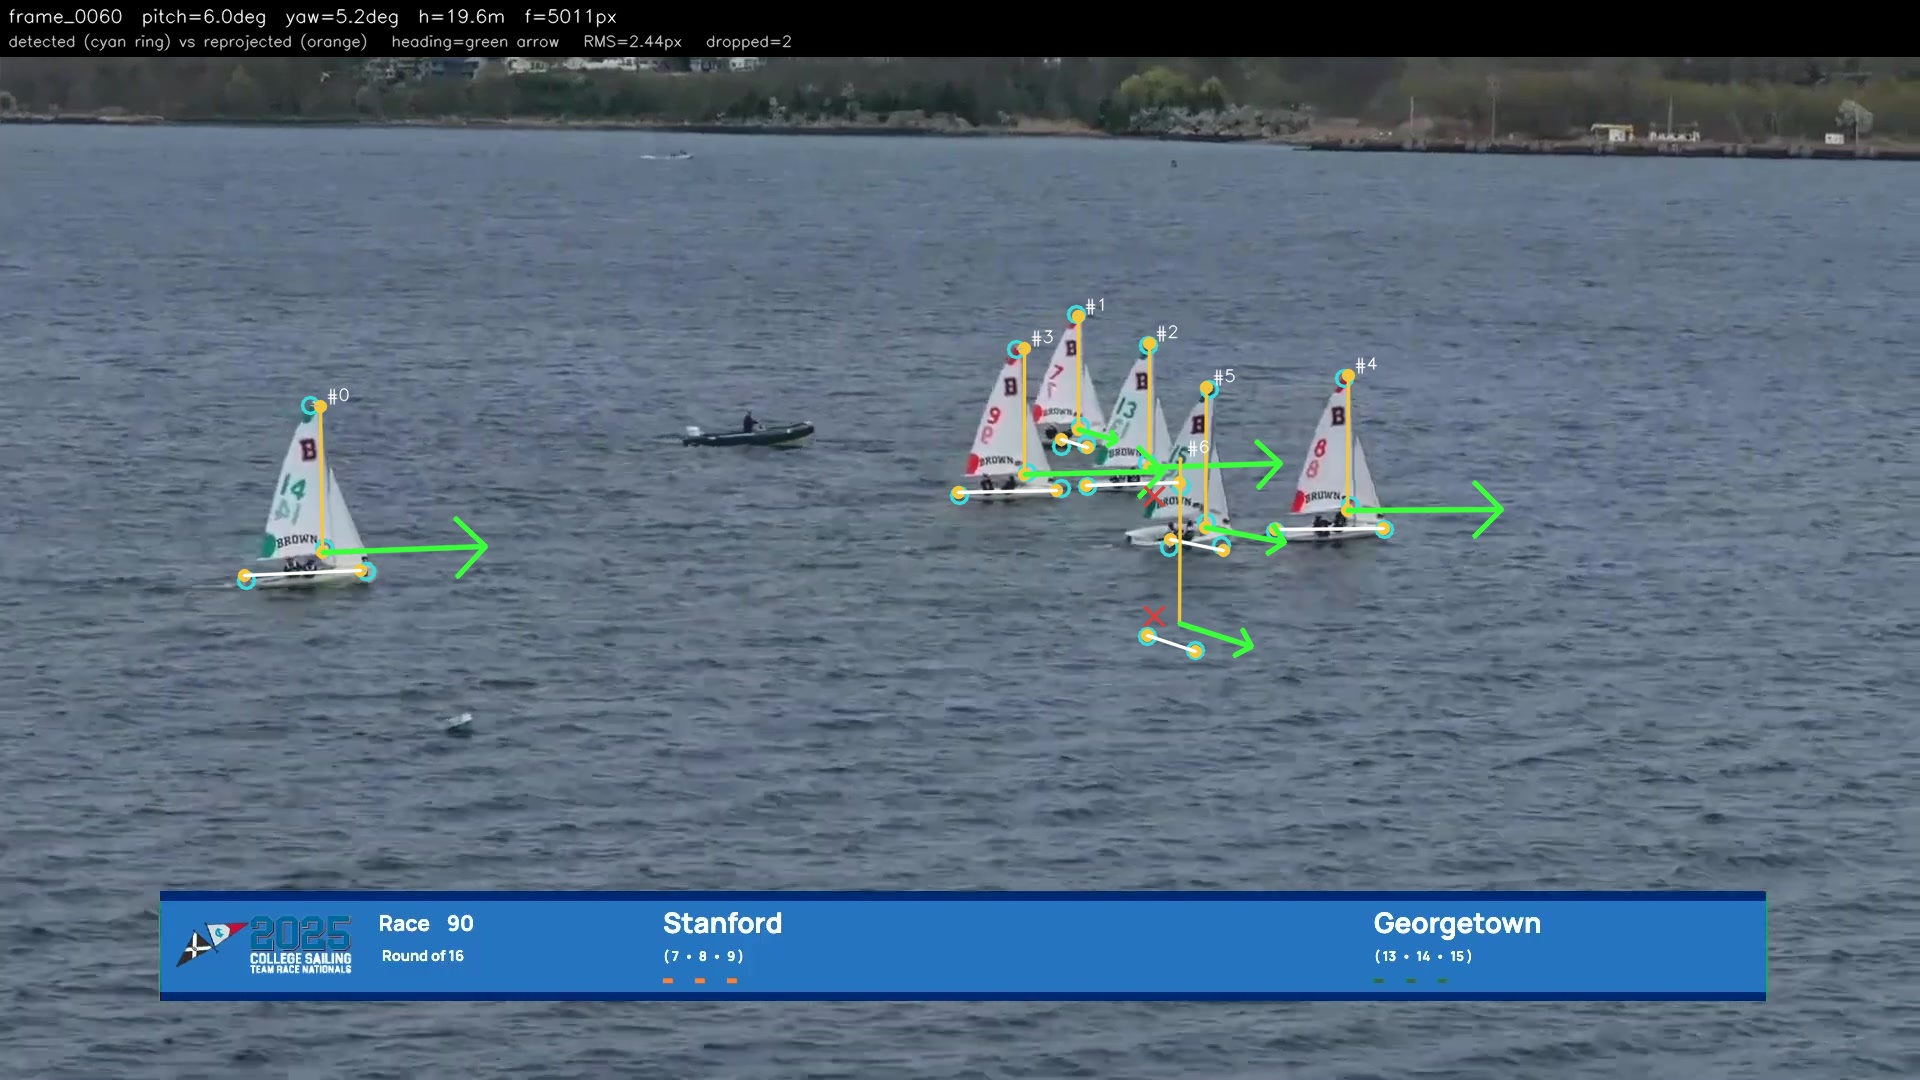
\includegraphics[width=\linewidth]{figure_solve_overlay.jpg}
    \caption{Per-frame solve overlay (frame 0060, 7 boats, RMS 2.44\,px).  Cyan rings are detected keypoints; orange dots are reprojections from the per-frame fit; green arrows show recovered heading.  White lines connect bow$\leftrightarrow$stern hulls and cyan lines mark the masts.}
    \label{fig:result1b}
\end{figure}

\subsection{Per-Frame Solve Quality and Top-Down View}

Each frame is solved independently --- the camera's pitch, yaw, height, focal length, and horizontal position are recovered fresh from the multi-boat reprojection constraint, and so is each boat's $(x, y, \mathrm{yaw}, \mathrm{heel})$.  Because the metric scale is baked into the boat template, the per-boat $(x, y)$ output of every frame is in metres in a world frame defined by the camera, immediately suitable for a per-frame top-down rendering of the fleet.

\subsection{Technical Discussion}

The most interesting empirical finding is how well the multi-boat geometric constraint conditions the per-frame problem.  PnP with unknown focal length is ill-posed for a single rigid object --- moving the object farther and zooming in produces nearly identical pixel patterns --- but six or seven boats simultaneously project through the same camera, and consistency of every boat's hull and mast under one shared $(\text{pitch}, \text{yaw}, h, f)$ is a much stronger constraint than any single boat alone provides.  This is why the per-frame solve is well-conditioned even with $f$ free, and why we did not need any temporal coupling.

The cascaded conditioning structure of the detector heads also matters more than the architecture would suggest.  A flat detector that predicts all four keypoints independently is less stable than one that predicts the tip first, then the base conditioned on tip context, then bow/stern conditioned on tip+base context.  Each subsequent stage gets a tighter spatial prior, and errors do not compound the way they do in flat detectors.

\section{Conclusion}

We presented an end-to-end pipeline that turns a monocular sailing broadcast into metric per-frame camera pose plus per-boat $(x, y, \mathrm{yaw}, \mathrm{heel})$, with median reprojection error of 3.88\,px and 100\% solve yield on a 43-second held-out clip.  The two ingredients that mattered most were a frozen DINOv3 backbone for visually-clean feature extraction and a multi-boat per-frame solver that exploits the geometric over-determination of having many rigid objects in one shared camera.  The result suggests that off-the-shelf broadcast footage is a viable substrate for automated tactical analysis of collegiate team racing without specialised hardware or GPS.

{\small
\bibliographystyle{plain}
\bibliography{ProjectFinal_ProjectReportTemplate}
}

\section*{Appendix}

\subsection*{Team contributions}

\begin{description}
\item[Quinn Brighton] Designed and trained the three-stage keypoint detection cascade (DINOv3 feature extraction, \texttt{TileHead}, \texttt{TipAttnBaseHead}, \texttt{TipBaseBowSternAttnHead}); implemented the per-frame least-squares solver (\texttt{solver\_clean.py}, \texttt{solve\_camera\_from\_frame.py}, \texttt{solve\_camera\_seq.py}) with iterative outlier rejection; engineered the end-to-end \texttt{run\_full\_pipeline.sh} script and per-frame visualization renderer.
\item[Nishani Clarke] Hand-labeled the initial bow/stern training set (261 pairs across 42 frames); audited and cleaned up training data; ran the comparative experiments across different training-data subsets used to pick the deployed model.
\item[Alexandra McIntyre] Hand-labeled the mast tip/base training set (1236 pairs across 200 frames); built the world-space top-down render of boat tracks and the per-frame topdown diagnostic; led the Related Work and Technical Discussion sections of this report.
\end{description}

\end{document}
